\newpage
\begin{flushleft}
  \textbf{\large 1 Задача отслеживания объектов на видеоизображениях}
\end{flushleft}
\refstepcounter{chapter}
\addcontentsline{toc}{chapter}{1 Задача отслеживания объектов на видеоизображениях}

Задача отслеживания объектов на видеоизображениях является одной из наиболее популярных среди исследователей в области компьютерного зрения. 
В этой главе будет представлено основывающееся на обзоре \cite{du2024exploring} краткое описание различных ее постановок, актуальности и проблем. 


\section{Постановка задачи}
В общем случае задача подразумевает работу с видеоизображением с целью получения информации о объектах и разбивается на три цели:
детектирование объектов в поле зрения, присвоение каждому из них уникального номера для идентификации и последующая запись истории перемещения. Способы их достижения разделяются на несколько основных подходов:
\begin{itemize}
    \item[--] MOT (англ. Multiple Object Tracking -- отслеживание нескольких объектов одновременно) или SOT (англ. Single Object Tracking -- отслеживание одного объекта);
    \item[--] работающие по мере поступления новых кадров (англ. online) или сразу со всем видео (англ. offline);
    \item[--] использование двухкомпонентных (нейронная сеть детектор в сочетании с алгоритмом отслеживания, который работает с показаниями детектора) или однокомпонентных (единая сеть, которая сразу детектирует и отслеживает) систем;
    \item[--] в случае двухкомпонентных систем: использующие ReID модели (англ. Re-identification -- дополнительная нейронная сеть, задачей которой является исключительно создание векторов значений (англ. embedding), позволяющих отличить объекты одного класса друг от друга) или работающие без них.
\end{itemize}

В ходе работы будут рассмотрены только двухкомпонентные MOT алгоритмы. Это связано с тем, что требования к вычислительным мощностям у них меньше, что является однозначным плюсом для запуска на маломощных устройствах.
Более того, двухкомпонентные алгоритмы самые универсальные с точки зрения применения готовых решений -- для адаптации под новый набор данных достаточно переобучить сеть классификатор.
Совокупность простоты использования и относительно низких вычислительных затрат выгодно выделяет этот класс алгоритмов и делает их идеальным выбором для множества областей, например, робототехники.

\section{Основные проблемы при решении задачи}
При решении поставленной задачи, возникает множество проблем. Среди них можно выделить следующие основные:
\begin{itemize}
    \item[--] пересечение объектов на изображении (например, люди в толпе), из-за чего системы испытывают трудности с сохранением присвоенных ранее уникальных номеров;
    \item[--] компенсация движения камеры;
    \item[--] изменения условий освещения, погоды или любых иных визуальных помехах;
    \item[--] проблемы реидентификации из-за схожести объектов одного класса;
    \item[--] проблемы реидентификации при временной потере объекта из поля зрения камеры;
    \item[--] баланс между производительностью и качеством работы;
    \item[--] работа в реальном времени и задержки обработки.
\end{itemize}

В ходе данной работы, основной фокус будет сделан на проблемах связанных с производительностью и задержками, а также запуске алгоритмов в реальном времени на малопроизводительных устройствах. 
Исследование данного вопроса поможет выработать общие рекомендации по выбору метода в зависимости от условий задачи (количество отслеживаемых объектов, качество видео и желаемая частота обновления), а также в целом проанализировать готовность технологии на данный момент к развертыванию на портативных устройствах.

\section{Актуальность}
Методы отслеживания объектов на видеоизображениях находят свое применение в самых разнообразных областях. 
Удешевление стоимости вычислений позволяет их использовать для все большего количества задач, например:
\begin{itemize}
    % \item[--] в системах помощи водителю или беспилотных автомобилях, для отслеживания движений пешеходов и других участников дорожного движения \cite{liu2025vehicle};
    \item[--] в спортивной аналитике, для более глубокого анализа аспектов игр, например, траекторий мяча \ref{fig:ball_track};
    \begin{figure}[ht]
        \centering
        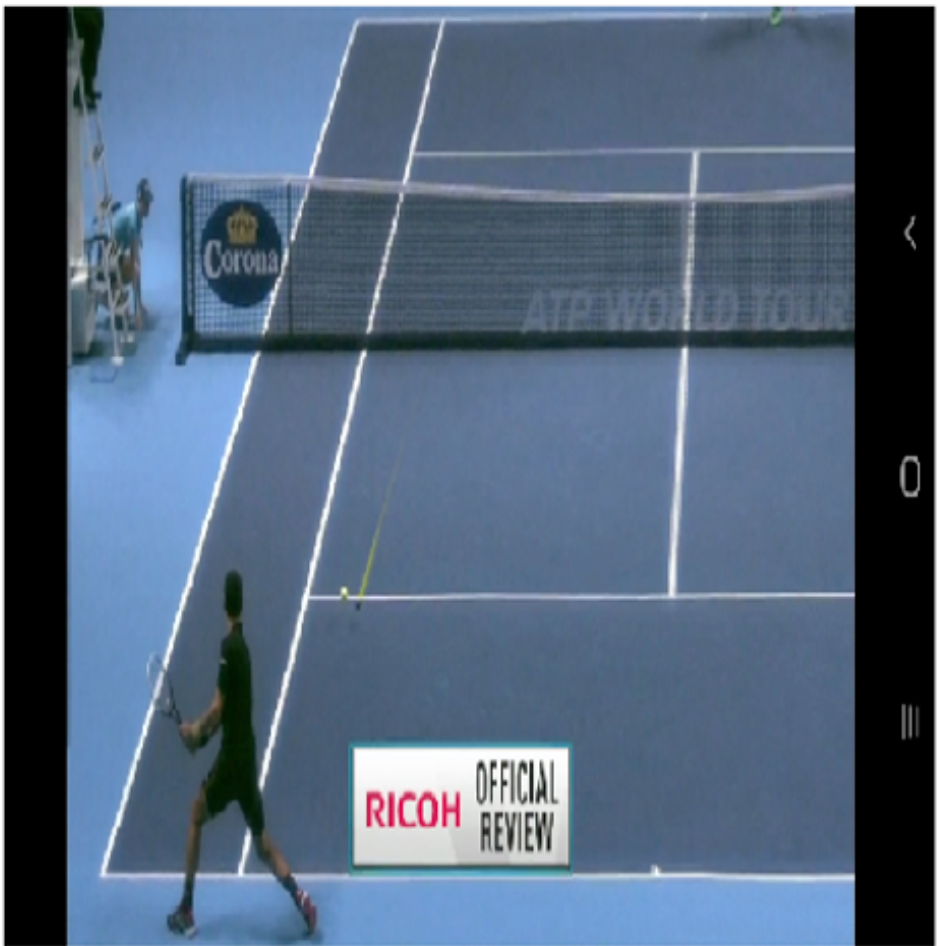
\includegraphics[width=0.7\textwidth]{review/ball_track.png}
        \caption{Пример отслеживания мяча в игре теннис \cite[страница 30, рисунок 16]{naik2022comprehensive}}
        \label{fig:ball_track}
    \end{figure}
    \FloatBarrier
    \item[--] в зоологии, для анализа поведения животных \ref{fig:animals}; 
    \begin{figure}[ht]
        \centering
        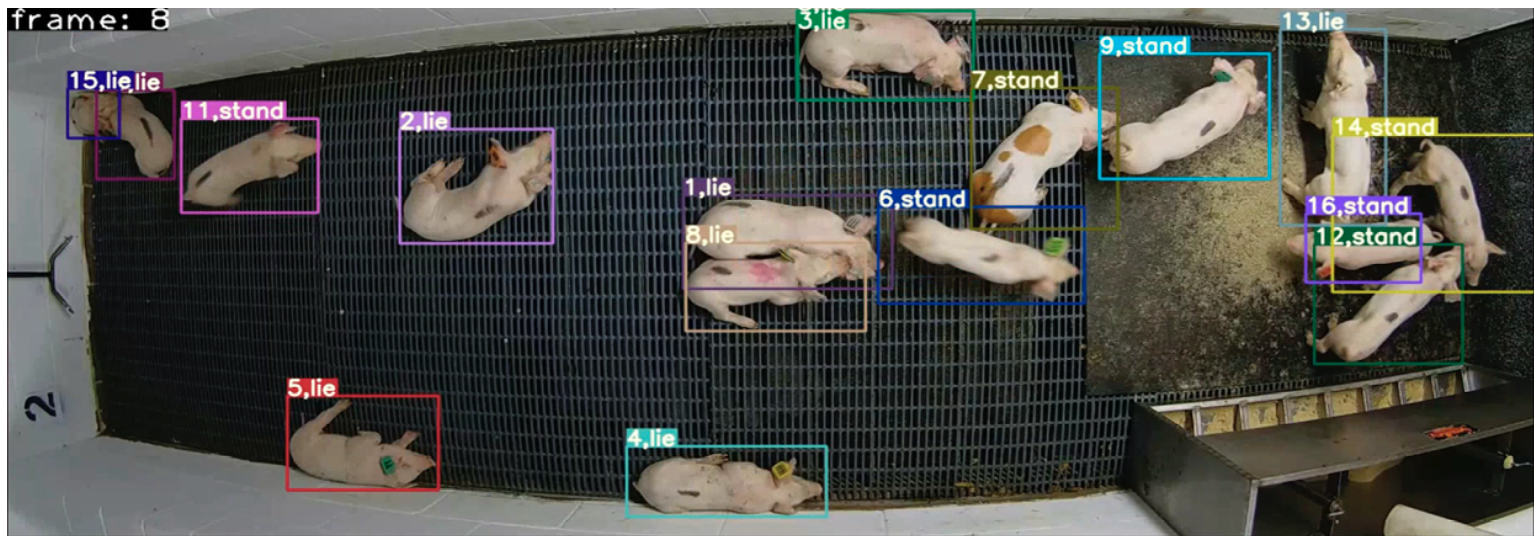
\includegraphics[width=0.7\textwidth]{review/animals.png}
        \caption{Пример отслеживания поведения свиней \cite[страница 12, рисунок 7]{tu2024behavior}}
        \label{fig:animals}
    \end{figure}
    \FloatBarrier
    \item[--] в урбанистике, для анализа паттернов передвижения или подсчета количества автомобилей \ref{fig:urban};
    \begin{figure}[ht]
        \centering
        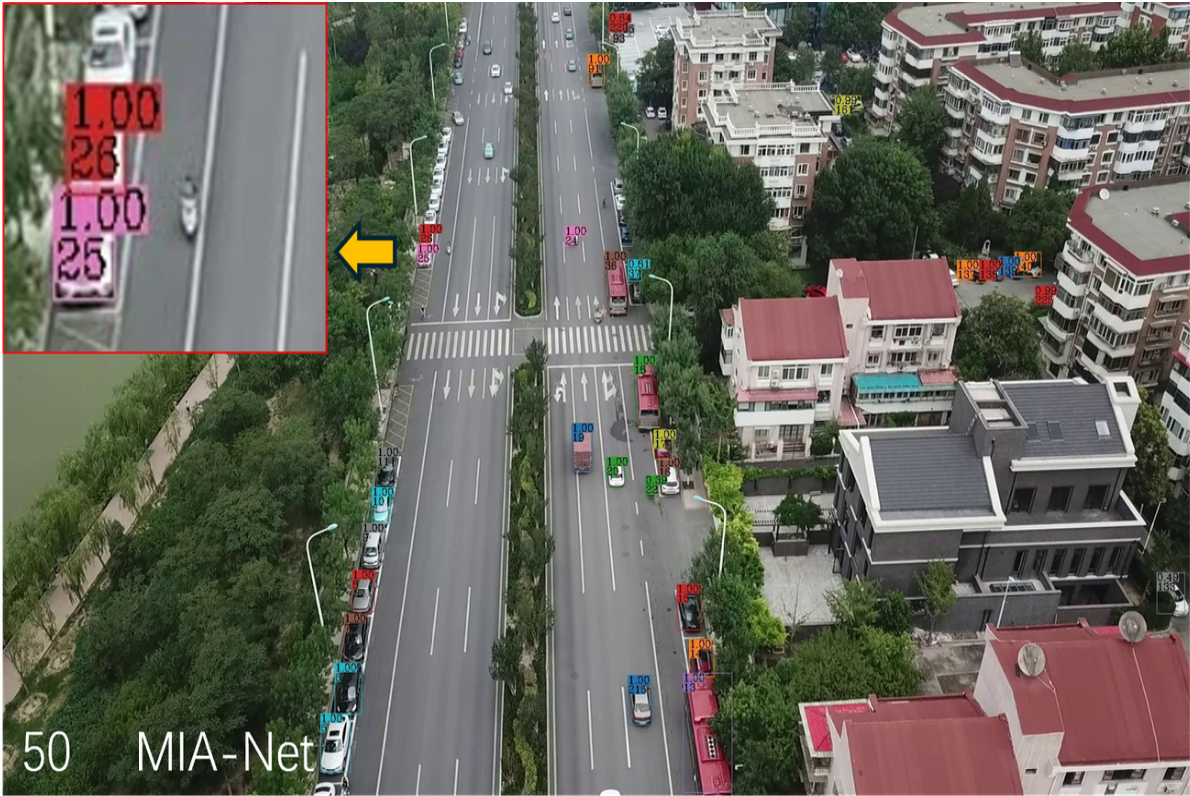
\includegraphics[width=0.7\textwidth]{review/urban_uav.png}
        \caption{Пример подсчета количества автомобилей с использованием дрона \cite[страница 16, рисунок 8]{wu2024multi}}
        \label{fig:urban}
    \end{figure}
    \FloatBarrier
    \item[--] в робототехнике, для отслеживания объекта \ref{fig:urban}. 

    % \item[--] для обеспечения безопасности и детектирования чрезвычайных ситуаций по информации с камер наружного наблюдения \cite{antony2024advancing};
    % \item[--] в фотосъемке, для удерживании в кадре объекта интереса \cite{gemerek2019video};  
    % \item[--] в розничной торговле, для анализа проведения покупателей и оптимизации раскладки товаров на стеллажах и витринах \cite{hossam2024revolutionizing};
\end{itemize}

C увеличением доступности технологии естественным образом будет расти и количество способов использования. 
В свою очередь, это будет приводить к возрастанию производительности труда, развитию отраслей с возрастающей отдачей и экономики -- повышению качества жизни.
Именно поэтому данная работа ставит своей целью изучить возможности запуска методов отслеживания объектов на видеоизображениях на малопроизводительных устройствах. 

\section{Выводы по главе}
В первой главе была рассмотрена постановка задачи отслеживания объектов на видеоизображениях. Представлены основные современные парадигмы решения задачи,
их основные отличия, а также выбрана наиболее перспективная для запуска на маломощных устройствах. 

Показана актуальность технологии и важность исследования поставленной цели, решение которой потенциально полезно для множества отраслей экономики.

В следующих главах будут более подробно рассмотрены принципы работы современных методов отслеживания, рассмотрены метрики оценивания показателей качества, набор данных, на которых будет проводиться сравнение.